\documentclass[crop,tikz]{standalone}

\tikzset{>=latex}

\begin{document}
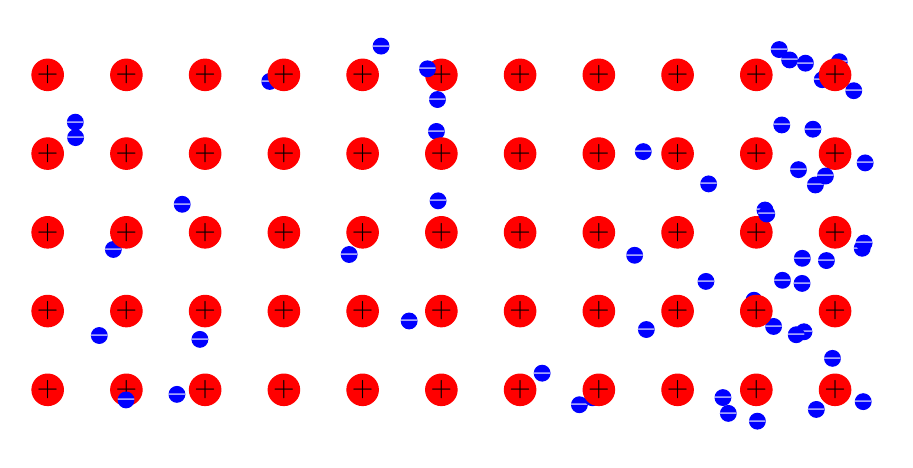
\begin{tikzpicture}
  \pgfmathsetmacro{\xmax}{10}
  \foreach \x in { 0,...,\xmax } {%
    \foreach \y in { 0,...,4 } {%
      \draw[fill,red] (\x,\y) circle (0.2) node[black] {$+$};
      \draw[fill,blue] ({\xmax*(1-abs(rand)^3)},\y)++(rand*180:0.4) circle (0.1) node[white] {$-$};
    }
  }
\end{tikzpicture}
\end{document}
